% !TEX encoding = UTF-8
% !TEX TS-program = pdflatex
% !TEX root = ../tesi.tex

%**************************************************************
\chapter{Progettazione e codifica}
\label{cap:progettazione-codifica}
%**************************************************************

\intro{In questo capitolo verranno spiegate le tecnologie utilizzate per lo sviluppo e l'architettura del prodotto software}\\

%**************************************************************
\section{Tecnologie e strumenti}
\label{sec:tecnologie-strumenti}

Di seguito viene data una panoramica delle tecnologie e strumenti utilizzati per lo sviluppo delle maschere e per la collaborazione con i colleghi stagisiti ed il tutor aziendale.

\subsection{Tecnologie}

\subsubsection*{Vue.js}
\begin{figure}[H]
	\begin{center}
		
\includegraphics[width=0.7\columnwidth]{vue.png}
		\caption{Logo di Vue.js}
	\end{center}
\end{figure}
Vue.js è un framework javascript open source nato nel 2013 che presenta un'architettura adottabile in modo incrementale che si concentra sulla composizione dei componenti, inoltre sono presenti funzionalità avanzate offerte tramite librerie e pacchetti di supporto. I componenti Vue estendono gli elementi HTML di base per incapsulare del codice riutilizzabile quindi a livello generale i componenti sono elementi personalizzati a cui il compilatore Vue associa una particolare funzionalità.\\
Vue utilizza quindi una sintassi basata su HTML e consente di associare il DOM renderizzato ai dati dell'istanza di Vue sottostante. In questo modo i modelli Vue possono essere analizzati da browser e parser HTML conformi alle modifiche ed inoltre con il sistema di reattività Vue è in grado di calcolare il numero minimo di componenti per eseguire nuovamente il rendering applicando la quantità minima di manipolazioni DOM quando cambia lo stato dell'app. Vue presenta un sistema reattivo grazie all'utilizzo di oggetti semplici Javascript ed ad un re-rendering ottimizzato: ogni componente durante il render tiene traccia delle sue dipendenze in modo tale che il sistema sappia quando e di quali componenti deve effettuare nuovamente il render.\\
Un problema che afflige le web application a pagina singola è che quest'ultime forniscono agli utenti la risposta basata solamente sull'URL dal server, di conseguenza l'utilizzo dei segnalibri a determinate schermate e la condivisione dei collegamenti a sezioni specifiche risulta molto difficile se non impossibile. Vue.js per riuscire a risolvere questo problema fornisce un'interfaccia, detta router, che da la possibilità di modificare ciò che viene visualizzato sulla pagina in base all'URL indipendentemente da come esso viene modificato. Infatti Vue.js viene fornito con il pacchetto open source "vue-router" che fornisce un'API per aggiornare l'URL dell'applicazione, supportare la cronologia di navigazione e le reimpostazioni di email e password. Tramite questa tipologia di router i componenti devono essere mappati alla route a cui appartengono per indicare dove deve essere eseguito il loro render.\\
Questo framework implementa il pattern MVVM, acronimo per Model-View-View-Model, una declinazione del più famoso MVC, ovvero Model-View-Controller. I componenti del MVVM sono:
\begin{itemize}
	\item Model (o Modello): l'implementazione del dominio dati come per il classico Modello del pattern MVC;
	\item View (o Vista): il componente grafico renderizzato dall'utente formato da HTML e CSS;
	\item ViewModel (o Vista per il Modello): il collante tra gli altri due componenti, esso fornisce alla View i dati in formato consono alla rappresentazione ed il comportamento di alcuni elementi dinamici.
\end{itemize}
La grossa differenza tra il pattern implementato da Vue.js e il Model-View-Controller sta nella differenza tra Controller e ViewModel. Il primo, infatti, è una porzione di codice che gestisce la logica di business grazie al Model e ritorna una View da mostrare all'utente; il secondo, invece, rappresenta una versione parallela al Model che risulta essere legato alla View e descrive il comportamento di quest'ultima con funzioni associate. Quindi mentre il Controller esegue logiche di business prima del rendering della View, il ViewModel definisce il comportamento dell'applicazione a runtime.

\subsubsection*{Vuetify}
Vuetify è un framework UI completo costruito su Vue.js nel 2014 ed il suo obiettivo è fornire agli sviluppatori gli strumenti per poter creare esperienze utente ricche e coinvolgenti. A differenza di altri framework Vuetify è progettato da zero in modo tale da renderlo facile da imparare ed essere gratificante da padroneggiare con centinaia di componenti realizzate dalle specifiche di Material Design.\\
Un pregio di questo framework è che adotta un approccio al mobile, questo significa che la web application sviluppata tramite esso sarà pienamente utilizzabile immediatamente su un tablet, un telefono ed un computer. Inoltre è un framework in sviluppo attivo che viene aggiornato settimanalmente rispondendo ai problemi e relativi report della community. Un altro pregio è, come si può vedere nell'immagine sottostante, il gran numero di funzionalità che possiede Vuetify in confronto agli altri framework di Vue.
\begin{figure}[H]
	\begin{center}
		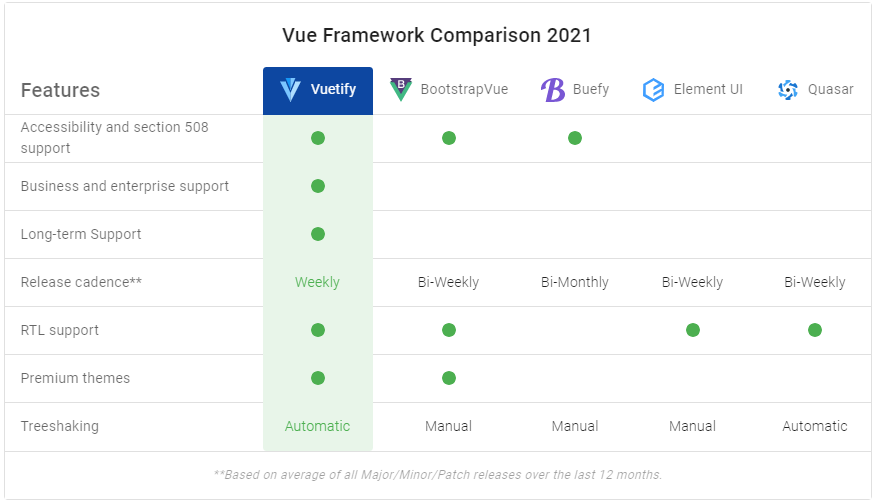
\includegraphics[width=1\columnwidth]{vuetify.png}
		\caption{Funzionalità di Vuetify}
	\end{center}
\end{figure}

\subsubsection{Vuex}

\subsection{Strumenti}

\subsubsection{Github}

Github è un servizio web e cloud-based fondato nel 2008 che aiuta gli sviluppatori ad archiviare, gestire il codice, tracciare e controllare le modifiche. I due argomenti principali legati a Github sono: controllo versioni e Git.\\
Il controllo versioni aiuta a tracciare e gestire le modifiche del codice di un progetto software: più un progetto risulta essere di grandi dimensioni più il controllo delle versioni diventa fondamentale. Infatti questo aiuta gli sviluppatori a lavorare con sicurezza attraverso due azioni:
\begin{itemize}
	\item branching: uno sviluppatore duplica parte del codice sorgente, detto repository, in modo da apportare modifiche in modo sicuro senza influenzare l'intero progetto;
	\item merging: una volta che lo sviluppatore è certo di aver prodotto del codice funzionante può fondere quel codice nel quello sorgente e renderlo ufficiale.
\end{itemize}
In questo modo tutte le modifiche possono essere monitorate e, se necessario, ripristinate. Inoltre grazie a questi concetti è possibile lavorare sullo stesso progetto in diversi sviluppatori senza problemi di ripetizioni di codice o conflitti durante lo sviluppo.\\
Git è un sistema di controllo verisoni distribuito realizzato nel 2005, ovvero l'intero codice base e la cronologia sono disponibili sul computer di ogni sviluppatore. In questo modo è possibile creare facilmente ramificazioni e fusioni.\\
Per organizzare il lavoro abbiamo creato un'\textit{organization}, prodotto offerto da Github che rende più semplice la collaborazione su più progetti contemporaneamente. Infatti ogni stagista ha creato la propria repository all'interno di questo spazio comune in modo tale da lavorare con i colleghi contemporaneamente e dare la possibilità ai tutor aziendali di visionare il lavoro svolto.

\subsubsection{Figma}

Figma è uno strumento nato nel 2016 rivolto ai web designer che hanno bisogno di un tool per la progettazione di interfacce. I vantaggi offerti da questo strumento sono i seguenti:
\begin{itemize}
	\item accessibilità multipiattaforma
	\item sistema di collaborazione in real-time
	\item utilizzo degli strumenti responsive oriented per una progettazione ottimale
	\item lavora in vettoriale
\end{itemize}
Grazie a questo strumento io e gli altri stagisti legati all'ambito front end abbiamo potuto creare dei prototipi delle maschere che avremmo dovuto sviluppare.

\subsubsection{Stoplight}

Stoplight è una piattaforma di progettazione \gls{api} collaborativa che si integra perfettamente nei flussi di lavoro per consentire a chiunque lavori con le \gls{api} di essere più produttive. Questa piattaforma si basa su tre principi guida fondamentali, in modo da essere responsabili, collaborativi e con intenti positivi. I principi sono i seguenti:
\begin{itemize}
	\item quando si vede un'opportunità per avere un impatto, bisogna coglierla;
	\item bisogna confidare l'uno nell'altro per aggiungere valore e risolvere problemi attraverso il lavoro di squadra;
	\item bisogna cercare di capire gli altri ascoltando, indagando e rispondendo con attenzione.
\end{itemize}
Grazie a questa piattaforma si può aiutare gli utenti interni ed esterni ad integrarsi rapidamente alll'\gls{api} di un altro utente pubblicando documentazione interattiva, tutorial ed esempi di codice sempre aggiornati.

\subsubsection{Visual Studio Code}

Visual Studio Code è un editor di codice sorgente sviluppato da Microsoft nel 2015. Esso può essere utilizzato con diversi linguaggi di programmazione, infatti incorpora in esso diverse funzioni che variano dal linguaggio con cui si sta programmando. Un punto di forza di questo editor è la sua graned malleabilità, infatti l'utente può installare o disinstallare diversi plugin in funzione del linguaggio che sta utilizzando.\\
Un altro punto di forza è la sua integrazione con Git facilitando il controllo di versione del lavoro svolto dal programmatore che ha la possibilità di controllare le modifiche fatte, risolvere eventuali conflitti e salvare il lavoro nella repository. Altri punti di forza di questo editor sono i seguenti:
\begin{itemize}
	\item IntelliSense, estensione che fornisce suggerimenti di completamento per variabili, metodi e moduli. In particolare per i metodi fornisce una breve spiegazione dei parametri che accettano e del loro funzionamento;
	\item Debug semplificato grazie ai plugin messi a disposizione e all'interfaccia grafica intuitiva;
	\item Modifica veloce delle righe di codice grazie ad avvisi su codice sospetto, possibilità di selezionare più righe contemporaneamente e suggerimenti sui parametri;
	\item Navigazione e refactoring del codice semplice.
\end{itemize}

%**************************************************************
\section{Ciclo di vita del software}
\label{sec:ciclo-vita-software}

%**************************************************************
\section{Progettazione}
\label{sec:progettazione}

\subsubsection{Namespace 1} %**************************
Descrizione namespace 1.

\begin{namespacedesc}
    \classdesc{Classe 1}{Descrizione classe 1}
    \classdesc{Classe 2}{Descrizione classe 2}
\end{namespacedesc}


%**************************************************************
\section{Design Pattern utilizzati}

%**************************************************************
\section{Codifica}
